%!TEX root = ../msc_thesis.tex

\chapter{Experimental results}
\label{ch:results}


\section{MNIST dataset}

The development so far has been to replicate \citeauthor{Gal2016Active}'s work done with MNIST dataset in \citetitle{Gal2016Active} and to implement two different architectures on a dataset provided by Amaury Gutiérrez that consists of pictures taken by drones before and after the September earthquake in three Mexican towns. Everything has been done in Keras using Tensorflow as backend and mainly through R, although some Python code was used via the \texttt{reticulate} package.

\subsection{Article replication}

My main goal in the replication  was to have an acquisition function that would outperform a random acquisition function. This was achieved and the results can be seen in figure \ref{fig:comparison_active_learning_random}, where one compare my results (on the left) with the original paper's results (right). The results are pretty similar overall, although the mean STD acquisition function was not implemented in the replication due to the bad performance shown in the paper.

Although my implementation achieved the goal of outperforming a random acquisition function, when comparing Bayesian and frequentist approaches the results differ. The paper's authors claim that the use of a Bayesian approach in the acquisition process of Active Learning leads to better accuracy with fewer images, but in my implementation there is virtually no distinction between both approaches. This can be seen in figures in \ref{fig:pred_entropy_AL} and \ref{fig:var_ratios_AL} that show my results (left) and the paper's authors results (right). In the paper, the frequentist acquisition functions show a worse performance than their Bayesian counterparts, but in my implementation there is no distinction. For example, with predictive entropy in figure \ref{fig:pred_entropy_AL}, the frequentist acquisition function in the original paper achieve a 90\% accuracy with around 300 images, while in my implementation this accuracy is first achieved with around 200 images.


\begin{figure}[H]
    \centering
    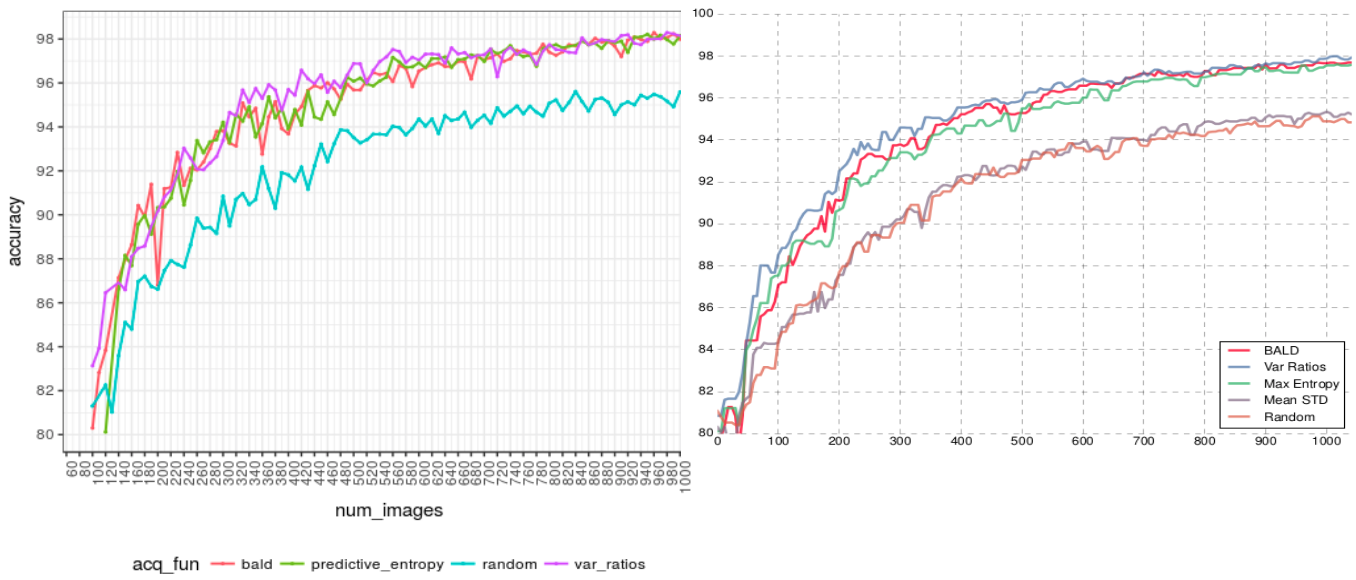
\includegraphics[width=\textwidth]{img_01.png}
    \caption{Accuracy of models in each acquisition step. The left picture shows my implementation and the right picture shows \citeauthor{Gal2016Active}'s implementation.}
    \label{fig:comparison_active_learning_random}
\end{figure}

\begin{figure}[H]
  \centering
  \subfloat[My results.]{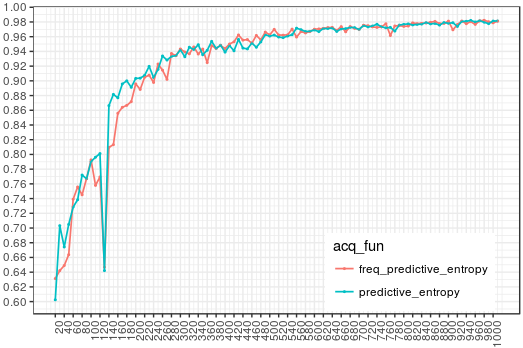
\includegraphics[width=0.5\textwidth]{pred_entropy_mine.png}}
  \hfill
  \subfloat[Paper's results.]{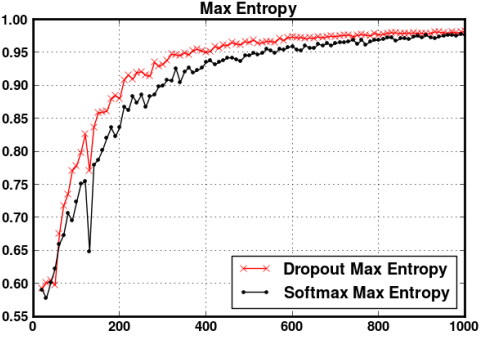
\includegraphics[width=0.5\textwidth]{pred_entropy_islam.png}}
  \caption{Accuracy of Bayesian and frequentist models in each acquisition step using predictive entropy as acquisition function. The left picture shows my implementation and the right picture shows \citeauthor{Gal2016Active}'s implementation.}
  \label{fig:pred_entropy_AL}
\end{figure}


\begin{figure}[H]
  \centering
  \subfloat[My results.]{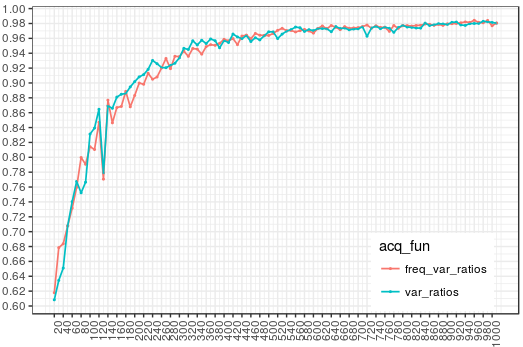
\includegraphics[width=0.5\textwidth]{var_ratio_mine.png}}
  \hfill
  \subfloat[Paper's results.]{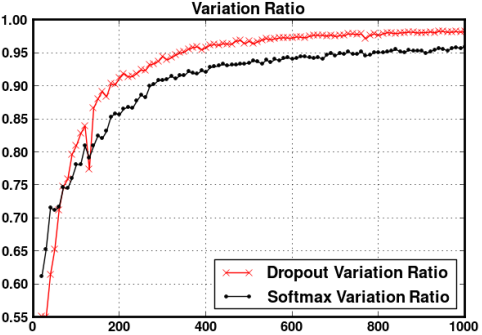
\includegraphics[width=0.5\textwidth]{var_ratio_islam.png}}
  \caption{Accuracy of Bayesian and frequentist models in each acquisition step using variation ratios as acquisition function. The left picture shows my implementation and the right picture shows \citeauthor{Gal2016Active}'s implementation.}
  \label{fig:var_ratios_AL}
\end{figure}

One more thing that should be mentioned is that I could not implement the BALD acquisition in the frequentist setting because of the way it is defined. The BALD uncertainty for a prediction $y$ given model parameters $\mathcal{W}$, features $x$ and training data $\mathcal{D}$ is defined as

\begin{equation}
	\label{eq:bald_def}
	\mathbb{I}[y, \mathcal{W} | x, \mathcal{D}] = \mathbb{H}[y | x, \mathcal{D}] - \mathbb{E}_{p(\mathcal{W} | \mathcal{D})}[\mathbb{H}[y | x, \mathcal{W}]]
\end{equation}

with $\mathbb{H}[y | x, \mathcal{D}]$ is the predictive entropy and is defined as $-\sum_c p(y = c | x, \mathcal{D}) \log p(y = c | x, \mathcal{D})$. In the Bayesian case, we have a set of $T$ dropout samples that approximate the predictive distribution, so the second part of equation \ref{eq:bald_def}, i.e., the expected value $\mathbb{E}_{p(\mathcal{W} | \mathcal{D})}[\mathbb{H}[y | x, \mathcal{W}]]$ is approximated by averaging the predictive entropy of each predictive sample; this way $\mathbb{I}[y, \mathcal{W} | x, \mathcal{D}]$ is computed by taking the difference of this quantity and the first part of equation \ref{eq:bald_def}. In the frequentist case, we only have one point estimate, so that difference is zero, so $\mathbb{I}[y, \mathcal{W} | x, \mathcal{D}]$ is zero for all points in the pool set. To this day, I don't know how the paper's authors computed it because their Github code is not clear and they haven't answered my email where I asked them that.
